\subsection{Building Generation}
The purpose of BuildingGenerator is to generate different kinds of visually pleasing buildings, everything from small houses to towering skyscrapers. 
The BuildingGenerator takes three inputs: the plot in which to build, the terrain on which to build on top of, and the population density that helps determine the size of the building \ref{table:buildinggen}.

\begin{table}[H]
  \centering
  \begin{tabular}{lllll}
    \textbf{Input}                           &               & \textbf{Function}            &               & \textbf{Output}         \\
    \midrule
    \textit{Plot, Terrain, Population}       & $\rightarrow$ & \textbf{BuildingGenerator}   & $\rightarrow$ & \textit{Building}       \\
    \bottomrule
  \end{tabular}
  
  \caption{Definition of the BlockGenerator function, which is responsible for constructing a single building on top of a plot.}
  \label{table:buildinggen} 
\end{table}
\vspace{-0.4cm} 

As buildings were considered a core part of a convincing modern city, it was essential to have a generator that could produce many different kinds of buildings. 
This problem was broken down into several sub-generators, each responsible for a particular type of building.
The plot label largely determined the sub-generator chosen for a specific plot.

% manhattan typ aktiga byggnader passar bra här
There two strategies used for generating buildings, the first of which used stochastic L-systems to generate diverse buildings.
The L-systems were implemented with type parameters to be able to handle the generation of many objects e.g. walls and floors.
The two types of parameters are the object type in the L-system and the data class that is used for the generation.
An example of the code to generate wall segments can be found in Figure \ref{fig:lsystem_example}.
A building generated via L-systems has some generated floors, where each floor has walls and is built with multiple smaller textured wall segments. 
These wall segments include windows, shop windows, and doors.

As an example, the steps for generating a Manhattan-style skyscraper are as follows:
\begin{enumerate}
    \item An L-system is used to generate different kinds of floors for the building. These floor types indicate what kind of L-system should be used later for the generation of the wall segments. Example of floor types include:
    \begin{itemize}
        \item FirstFloor - A floor that has shop windows and doors.
        \item OnlyWindowFloor - A floor that will only have window segments. 
        \item MirrorFloor - A symmetric floor where one half of the floor segments are copied and flipped to the other half.
    \end{itemize}
    These example types are visualized in Figure \ref{fig:segmentsgen}.
    \item Each wall is then generated, floor-by-floor. Each floor type has its own L-system to generate different wall segments.
    \item The walls are then put together inside the plot, with a flat roof on top.
    \item The building is then placed on the highest point of the terrain within the plot. Basement walls are then generated downwards to connect the building with the ground. %techically it's the highest point of the plot.points
\end{enumerate}

% Explain how the direction of the wall is decide. Maybe draw a picture of it?

\begin{figure}[H]
  \centering
  \begin{subfigure}[b]{0.32\textwidth}
    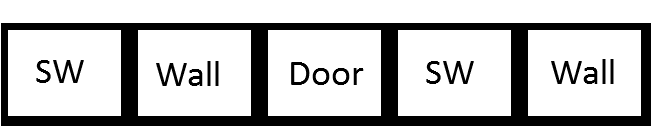
\includegraphics[width=\textwidth]{figure/FirstFloor.png}
    \caption{FirstFloor.}
  \end{subfigure}
  \quad
  \begin{subfigure}[b]{0.32\textwidth}
    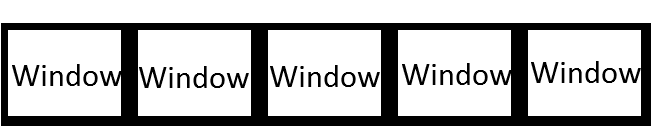
\includegraphics[width=\textwidth]{figure/OnlyWindowFloor.png}
    \caption{OnlyWindowFloor.}
  \end{subfigure}
  \begin{subfigure}[b]{0.32\textwidth}
    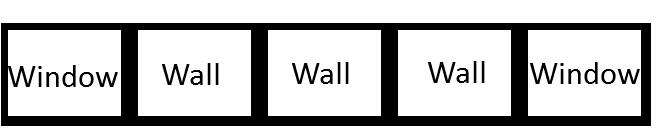
\includegraphics[width=\textwidth]{figure/MirrorFloor.png}
    \caption{MirrorFloor.}
  \end{subfigure}
  \caption{Three different floor types and an example of their wall segment generation.}
  \label{fig:segmentsgen}
\end{figure}

The second strategy was only applied to certain skyscrapers and used a large texture atlas of windows from which subregions of windows were randomly sampled.
These skyscrapers were also adjusted in size, depending on the population.
This strategy, although quite simple, provided useful variation for windows, which tend to look a bit too similar otherwise.

%du har en stor repeating texture, två olika sådana av textures, tar små delar av den här textures, och applicerar den på olika ställen av skyskrapan
%fönstrena blir slumptade. 
%random uv koordinat
%random subbild och applicerar det i ett grid. 

\begin{figure}[H]
  \begin{lstlisting}[]
    lSystem = new LSystem<ManhattanWallSegmentType, ManhattanSegmentsGeneratorData>();

    lSystem.ShouldContinue(value => value.widthLeft > 0);

    lSystem.CreateRules(Corner)
        .Add(0.5f, Wall)
        .Add(0.5f, Window)
        .OnAccepted(value => new ManhattanSegmentsGeneratorData(value.widthLeft - cornerWidth));

    lSystem.CreateRules(Window)
        .Add(0.5f, Wall)
        .Add(0.5f, Window)
        .ShouldAccept(value => value.widthLeft >= windowWidth)
        .OnAccepted(value => new ManhattanSegmentsGeneratorData(value.widthLeft - windowWidth));

    lSystem.CreateRules(Wall)
        .Add(0.5f, Wall)
        .Add(0.5f, Window)
        .ShouldAccept(value => value.widthLeft >= wallWidth)
        .OnAccepted(value => new ManhattanSegmentsGeneratorData(value.widthLeft - wallWidth));
  \end{lstlisting}
  \caption{Example of wall segment generation via L-System in code. Notice how the \textit{Wall} segment types have a 50\% chance of the next segment being another \textit{Wall}, or a \textit{Window}.}
  \label{fig:lsystem_example}
\end{figure}
